\documentclass[a4paper,11pt]{article}
\usepackage[catalan]{babel}
\usepackage{amsmath}
\usepackage{amsthm}
\usepackage{amssymb,units,mathtools,siunitx}
\usepackage[T1]{fontenc}
\usepackage{commath}
\usepackage{multicol}
\usepackage[a4paper]{geometry}
\addto{\captionscatalan}{\renewcommand{\abstractname}{Abstract}}
\geometry{top=3.75cm, bottom=3.00cm, left=2.50cm, right=2.15cm}
\usepackage[utf8]{inputenc}
\usepackage{graphicx}
\title{Pràctica 2. Força entre corrents}
\date{}


\begin{document}
\maketitle
\begin{abstract}
Aquest informe presenta els resultats de l'estudi de la força exercida entre dos corrents paral·lels pels quals hi circula la mateixa intensitat. Concretament, s'ha provat experimentalment la dependència lineal entre la força i el quadrat de la intensitat i entre la força i l'invers de la distància entre els fils.

A més, s'ha trobat experimentalment el valor de la constant $\mu_0$ assumint la llei de Biot-Savart, i obtenint $\mu_0=(1.25\pm0.04)\cdot10^{-6}\ \si{N/A^2}$ i $\mu_0=(3.0\pm0.4)\cdot10^{-6}\ \si{N/A^2}$. El primer valor és consistent amb el tabulat, mentre que el segon només n'és de l'ordre. 

Finalment, s'ha mesurat la component radial del camp magnètic terrestre, obtenint un valor de $B=(1.59\pm0.18)\cdot10^{-5}\ \si{T}$, de l'ordre del que descriuen altres articles.
\end{abstract}

\section{Introducció i Objectius}
L'objectiu principal d'aquesta pràctica és la comprovació experimental de la llei de Biot-Savart en el cas de dos fils paral·lels. S'ha calculat la força que s'exerceixen dos fils paral·lels pels quals hi circula la mateixa intensitat.

Més concretament, s'han avaluat experimentalment les correlacions entre la força entre els corrents i el quadrat de la intensitat que hi circula, i també entre la força i l'invers de la distància a què es troben.

 A més, s'ha determinat experimentalment la constant $\mu_0$ i el valor de la component radial del camp magnètic terrestre.

A partir de la llei d'Àmpere, es pot deduir que la força que s'exerceixen dos fils amb les característiques mencionades anteriorment és 

\begin{equation}
F=\frac{\mu_0I^2L}{2\pi r}
\end{equation}
on $I$ és la intensitat que hi circula, $L$ la longitud dels dos fils i $r$ la separació entre ells.

També, si existeix un camp $B$ constant al llarg de tot el fil, la força que sent aquest és

\begin{equation}
	F=BLI
\end{equation}

\section{Mètode experimental}
Totes les mesures s'han pres en una balança de corrents. La Figura 1 mostra un esquema del dispositiu, amb els elements principals.
\begin{figure}
	\centering
	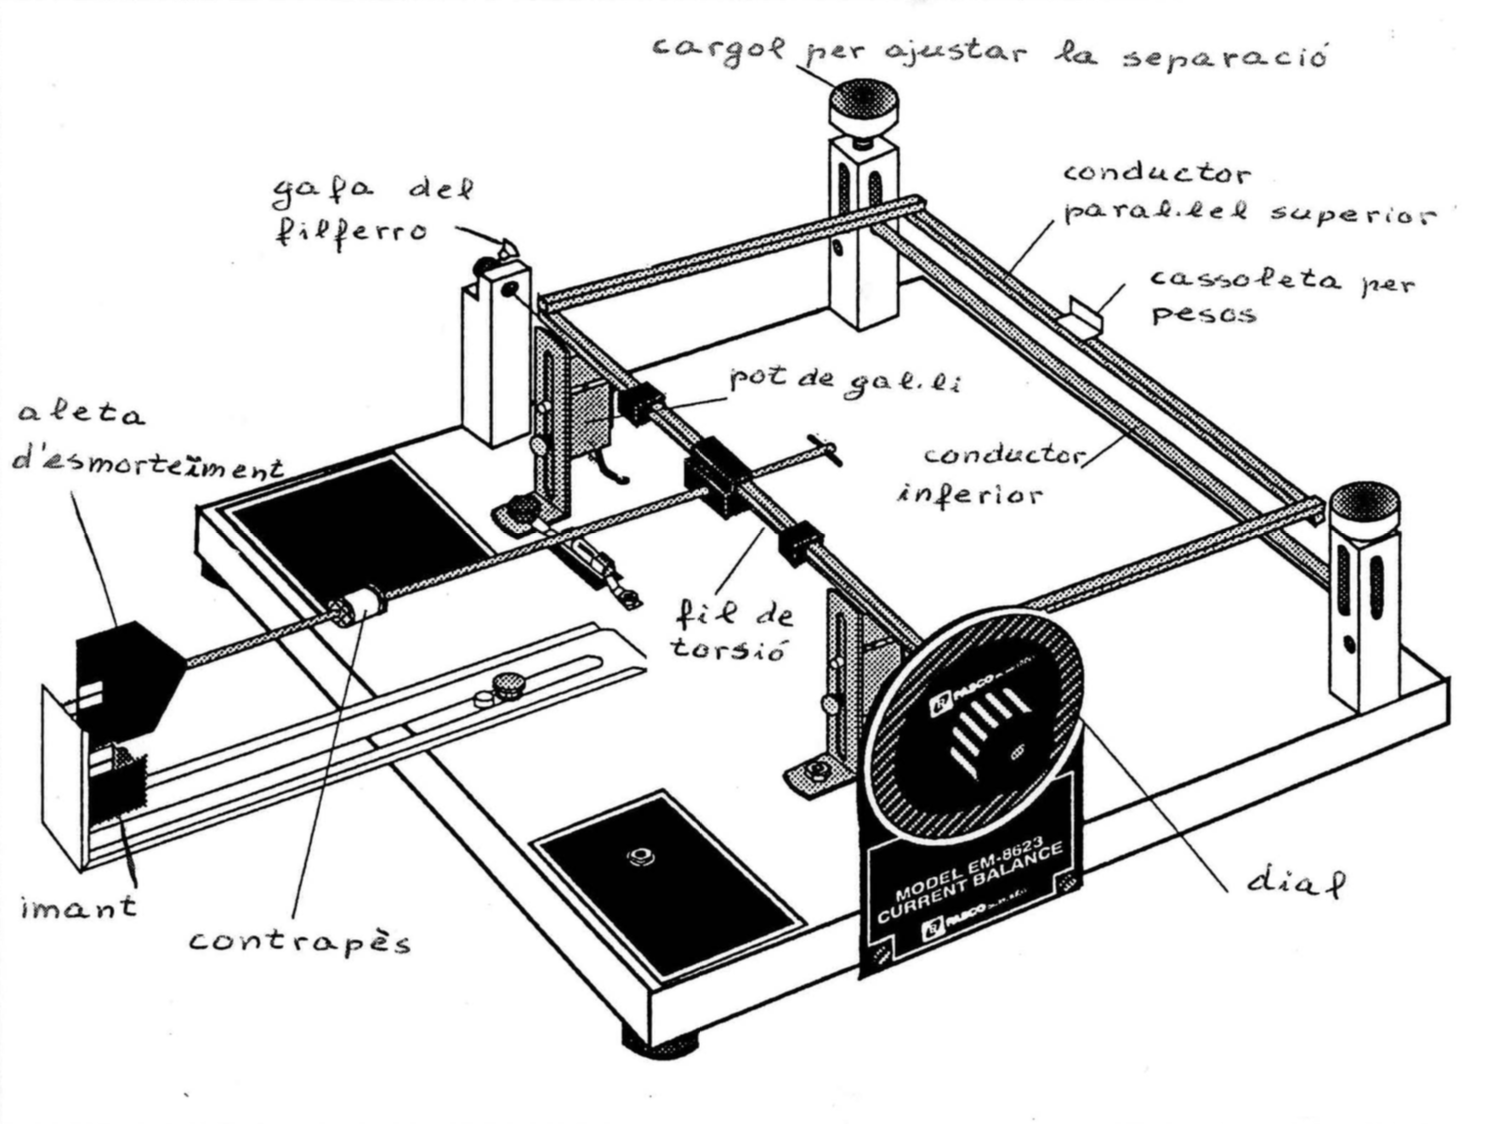
\includegraphics[scale=0.5]{Fig1.png}
	\caption{Esquema de la balança de corrents amb els principals elements}
\end{figure}

La balança disposa de dos maneres de determinar la força entre els corrents. Per una banda, disposa d'una cassoleta de pesos on col·locar diferents masses. Sabent que, en el moment que la balança es troba equilibrada, la força gravitatòria sobre la massa és igual a la força entre els corrents es pot determinar aquesta última. Per l'altra banda, la balança també disposa d'un dial i un fil de torsió que poden contrarrestar la força entre els corrents. Sabent que la relació entre els graus que rota el dial i la força que fa és lineal, i coneixent la constant de proporcionalitat es pot determinar també la força entre els corrents.

Creiem necessari comentar que els corrents s'han disposat en direcció nord-sud terrestre per tal que el camp magnètic de la Terra no influís en els nostres resultats.

Cal també comentar que el valor que s'ha pres com a acceleració de la gravetat és $9.80665 \si{m/s^2}$ sense incertesa, ja que s'ha considerat que és menyspreable enfront a la resta d'incerteses que puguem tenir. S'han pres també sense incertesa els valors de les masses proporcionades al laboratori.

\subsection{Força vs. Intensitat}

Per aquesta part de la pràctica s'ha mesurat la intensitat necessària per compensar la força gravitatòria exercida sobre el cable superior per masses de $5,\ 10,\ 15,\ 20$ i $25\si{mg}$. Posteriorment s'ha aplicat una regressió lineal entre la força i el quadrat de la intensitat per comprovar-ne la correlació predita per l'expressió 2.

\subsection{Força vs. Distància}
En aquesta part, s'ha fixat una intensitat i s'ha anat variant la distància entre els cables amb els cargols disposats amb aquest fi. Per cada distància desitjada s'ha determinat la força entre els corrents a partir del dial i el fil de torsió. A les dades preses se'ls hi ha aplicat una regressió lineal entre la força i l'invers de la distància de separació per comprovar la correlació predita per l'expressió 2. A partir del pendent obtingut en la regressió i l'expressió 2 s'ha determinat experimentalment la constant $\mu_0$.
\subsection{Camp Magnètic Terrestre}
Per aquesta part de l'experiència %Arnau I lof u
s'han orientat els corrents en direcció est-oest per tal que influís la component radial del camp magnètic terrestre. Per la disposició de la balança i el fet que la força que un camp magnètic exerceix sobre un corrent és perpendicular al pla que defineixen no es pot determinar la component horitzontal del camp magnètic terrestre.

Posteriorment, s'ha fet circular una intensitat fixa només pel fil superior i s'ha determinat la força que patia a través del dial i el fil de torsió. El camp magnètic s'ha determinat a partir de l'expressió 3.

\section{Resultats}
\subsection{Força vs. Intensitat}
La Taula 1 mostra les mitjanes de les intensitats necessàries per contrarrestar la força gravitatòria de les diferents masses usades. La Taula A2.1 % Jo denotaria aixi les coses de l'annex
de l'annex mostra totes les dades per a cada massa.

\begin{table}
	\centering
	\caption{Intensitat mitjana necessària per contrarrestar la força gravitatòria de cada massa.}
	\vspace{0.5cm}
	\begin{tabular}{|c|c|c|}
		\hline
		\textbf{Massa ($\si{mg}$)}&\textbf{Intensitat} $\si{(A)}$& \textbf{Incertesa en la intensitat} $\si{(A)}$\\ \hline
		5 & 2.62 & 0.10 \\ \hline
			10 & 3.62 & 0.18 \\ \hline 
				15 & 4.49 & 0.15 \\ \hline 
					20 & 5.19 & 0.18 \\ \hline 
						25 & 5.8 & 0,3 \\ \hline  
	\end{tabular}
\end{table}
Amb els valors presentats a la Taula 1 s'ha fet una regressió lineal entre la força entre corrents i el quadrat de la intensitat. La regressió, amb un coeficient $r^2=0.999$, es presenta a la Figura 2.

El valor obtingut del pendent de la recta de regressió es de $m=(7.35\pm0.08)\cdot10^{-6}\ \si{N/A^2}$. A partir d'aquest valor i l'expressió 2 s'ha determinat $\mu_0=(1.25\pm0.04)\cdot10^{-6}\ \si{N/A^2}$, que és compatible amb el valor tabulat.
\subsection{Força vs. Distància}
Primerament, a través d'una regressió lineal amb un factor de correlació $r^2=0.985$ s'ha determinat la dependència lineal entre la força exercida pel fil de torsió i la rotació del dial, amb un valor de la constant de proporcionalitat de $k=(3.2\pm0.2)\cdot10^{-7}\ \si{N/grau}$. Les dades de la regressió es poden veure a la Taula A2.2 i a la Figura A2.1, ambdues a l'annex. Així, la força es pot determinar per
\begin{equation}
	F=k\theta
\end{equation}

S'ha fixat una intensitat constant de $I=(5.37\pm0.02)\ \si{A}$ i s'ha mesurat la rotació necessària del dial per contrarrestrar la força entre corrents. La Taula 2 mostra els resultats.

\begin{table}
	\centering
	\caption{Rotació del dial necessària per contrarrestar la força entre corrents a diferents distàncies. La intensitat, fixa, és de $(5.37\pm0.02)\ \si{A}$.}
	\vspace{0.5cm}
	\begin{tabular}{|c|c|}
		\hline
		\textbf{Separació ($\si{m}$) ($\pm 0.001\ \si{m}$)}&\textbf{Rotació del dial} $\si{(º)}$ ($\pm 1º$) \\ \hline
		0.010 & 64  \\ \hline
		0.009 & 63  \\ \hline 
		0.008 & 65 \\ \hline 
		0.007 & 87  \\ \hline 
		0.006 & 129  \\ \hline  
		0.005 & 186  \\ \hline  
	\end{tabular}
\end{table}
Amb les dades de la Taula 2 s'ha realitzat una regressió lineal entre la força entre corrents, calculada a partir de l'expressió 3, i l'invers de la distància. La regressió, amb un coeficient $r^2=0.932$, es pot veure a la Figura 2.

El pendent obtingut a partir de la regressió és $n=(4.1\pm0.6)\cdot10^{-6}$. A partir d'aquest valor i l'expressió 2 s'ha determinat experimentalment el valor de la constant $\mu_0=(3.0\pm0.4)\cdot10^{-6}\ \si{N/A^2}$. El resultat no és consistent amb el valor tabulat, possiblement per interferències amb altres elements, però sí de l'orde del valor acceptat.

\subsection{Camp Magnètic Terrestre}
La Taula 3 mostra tres mesures d'intensitat i les respectives rotacions del dial per tal de compensar la força que el cable pateix degut a la component radial del camp magnètic terrestre. La força s'obté a partir de l'expressió 3, i el camp a partir de l'expressió 2.

\begin{table}
	\centering
	\caption{Mesures de la component radial del camp magnètic terrestre}
	\vspace{0.5cm}
	\begin{tabular}{|c|c|c|c|}
		\hline
		\textbf{Intensitat} $\si{(A)}$ $(\pm0.01\ \si{A})$&\textbf{Rotació del dial} $\si{(º)}$ ($\pm 1º$)&\textbf{Camp magnètic} $\si{(nT)}$ & \textbf{Incertesa} $\si{(nT)}$\\ \hline
		6.06 & 8 &$1.4\cdot10^{4}$ & $0.3\cdot10^{4}$ \\ \hline
		6.13 & 8  &$1.4\cdot10^{4}$  &$0.3\cdot10^{4}$ \\ \hline 
		6.57 & 12 &$2.0\cdot10^{4}$  &$0.4\cdot10^{4}$ \\ \hline 

	\end{tabular}
\end{table}
D'aquesta manera, obtenim, a partir de la mitjana aritmètica dels valors de la Taula 3, un valor de la component radial del camp magnètic terrestre de $B=(1.59\pm0.18)\cdot10^{-5}\ \si{T}$. El resultat no és consistent amb el valor tabulat del camp magnètic a Madrid l'any 1975, possiblement per interferències amb altres elements, però sí que n'és de l'ordre.

\section{Conclusions}
Concloem, primer de tot, que existeix una relació lineal entre la força exercida entre dos corrents com els descrits i el quadrat de la intensitat que hi circula, així com amb l'invers de la distància a què es troben, tal com prediu la llei de Biot-Savart.

A més, s'ha pogut determinar experimentalment l'ordre de la constant $\mu_0$ a partir de dues regressions lineals i l'assumpció que la llei de Biot-Savart és vàlida. Les possibles discrepàncies amb el valor real es creuen degudes a possibles interferències amb elements del laboratori o a errors sistemàtics.

Finalment, s'ha determinat també l'ordre del valor de la component radial del camp magnètic terrestre, que coincideix amb el valor tabulat. La component tangencial no s'ha pogut mesurar degut a la disposició de la balança.


\section*{Annex}

\begin{table}
	\centering
	\caption{HAURIA D'ESTAR DENOTADA PER TAULA A2.1!!! Mesures de la intensitat necessària per contrarrestar la força gravitatòria de cada massa}
	\vspace{0,2cm}
	\begin{tabular}{|c|||c||c||c||c||c|}
		\hline
		\textbf{Massa} $\si{(mg)}$ &\textbf{5}&\textbf{10}&\textbf{15}&\textbf{20}&\textbf{25} \\\hline
		\textbf{Mesura 1} $\si{(A)}$ $(\pm0.01\ \si{A})$&2.62&3.70&4.47&5.10&6.05\\\hline
		\textbf{Mesura 2} $\si{(A)}$ $(\pm0.01\ \si{A})$&2.55&3.40&4.46&5.29&5.99\\\hline
		\textbf{Mesura 3} $\si{(A)}$ $(\pm0.01\ \si{A})$&2.65&3.58&4.63&5.33&5.94\\\hline
		\textbf{Mesura 4} $\si{(A)}$ $(\pm0.01\ \si{A})$&2.62&3.64&4.42&5.07&5.40\\\hline
		\textbf{Mesura 5} $\si{(A)}$ $(\pm0.01\ \si{A})$&2.60&3.71&4.50&5.10&5.21\\\hline
		\textbf{Mesura 6} $\si{(A)}$ $(\pm0.01\ \si{A})$&2.57&3.68&4.48&5.11&5.63\\\hline
	\end{tabular}
\end{table}


\begin{table}
	\centering
	\caption{HAURIA D'ESTAR DENOTADA PER TAULA A2.2!!! Dades de la regressió lineal entre la força del fil de torsió i la rotació del dial}
	\vspace{0,2cm}
	\begin{tabular}{|c|c|}
		\hline
\text{Massa} $\si{mg}$ & \textbf{Rotació del dial $(º)$ $(\pm1º)$}\\ \hline
5 & 13 \\ \hline
10 & 27 \\ \hline
15 & 44 \\ \hline
20 & 63 \\ \hline
25 & 70 \\ \hline
	\end{tabular}
\end{table}



\end{document}
